\documentclass{article}

\usepackage{geometry}
\usepackage{amsmath}
\usepackage{graphicx}
\usepackage{amssymb}
\usepackage{hyperref}
\hypersetup{
  colorlinks=true,
  linkcolor=blue,
  citecolor=blue,
  urlcolor=blue
}
\begin{document}
    \begin{center}
        Letter for Referee
    \end{center}

    Dear referee and editor, \\

    We would like to thank the referee for their careful consideration of our work as well as their very insightful comments. We have modified the body of the paper in a way that hopefully address the points raised by the referee. Below, we list the referee's comments, discuss them and describe the modifications we made to the article: \\

    \textbf{Comment \#1:} "The authors modified camb-cs2 to calculate theoretical predictions for Horndeski models. I am wondering how their outputs compared with other public also more widely-used tools for such models e.g. EFTCAMB."\\

    \textbf{Answer \#1:} The implementation of CAMB-cs2 heavily relies on ISiTGR\footnote{\url{https://github.com/mishakb/ISiTGR}}: we copied the modification of the perturbation equations, but we stripped out most of the functionality to suit our models. To validate our code, we have reproduced results from the literature. For this purpose, we also have implemented the phenomenological $\mu_0-\Sigma_0$ parameterization, where the $\mu(a)$ and $\Sigma(a)$ functions are scale-independent and proportional to the relative dark energy abundance. Figure~\ref{fig:reproduction} below shows reproductions of Figures 3 and 4 of \href{https://arxiv.org/abs/1212.3339}{CFHTLenS: Testing the Laws of Gravity with Tomographic Weak Lensing and Redshift Space Distortions} and are generated using CAMB-cs2, and the original Figures were generated using MGCAMB. \\

    \begin{figure}
        \centering
        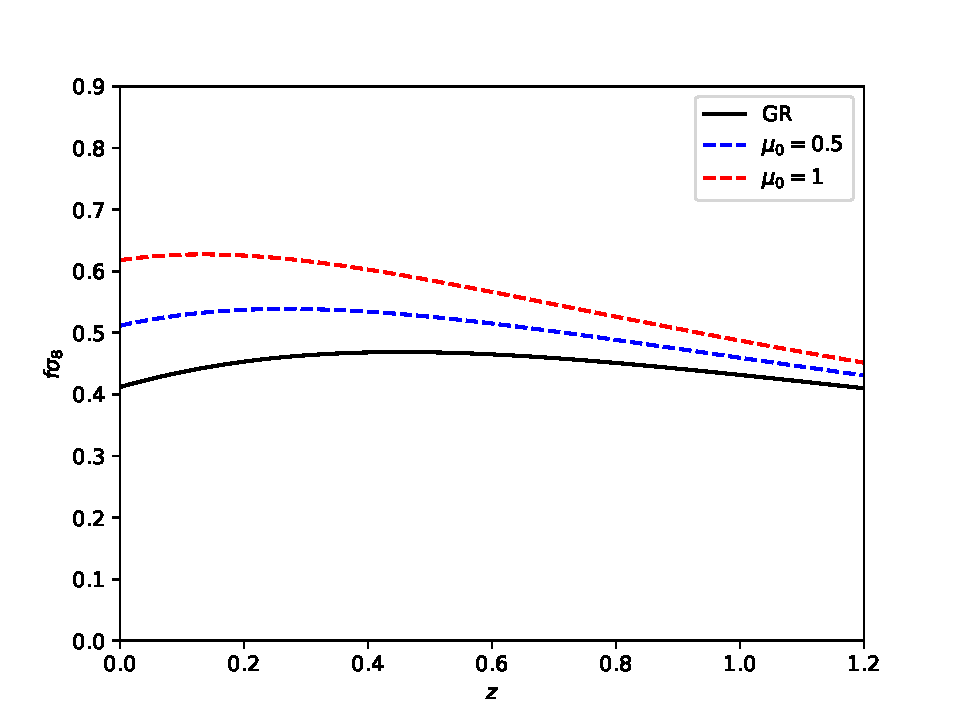
\includegraphics[width=0.5\linewidth]{figures/referee/Fig3_CFHT.pdf}
        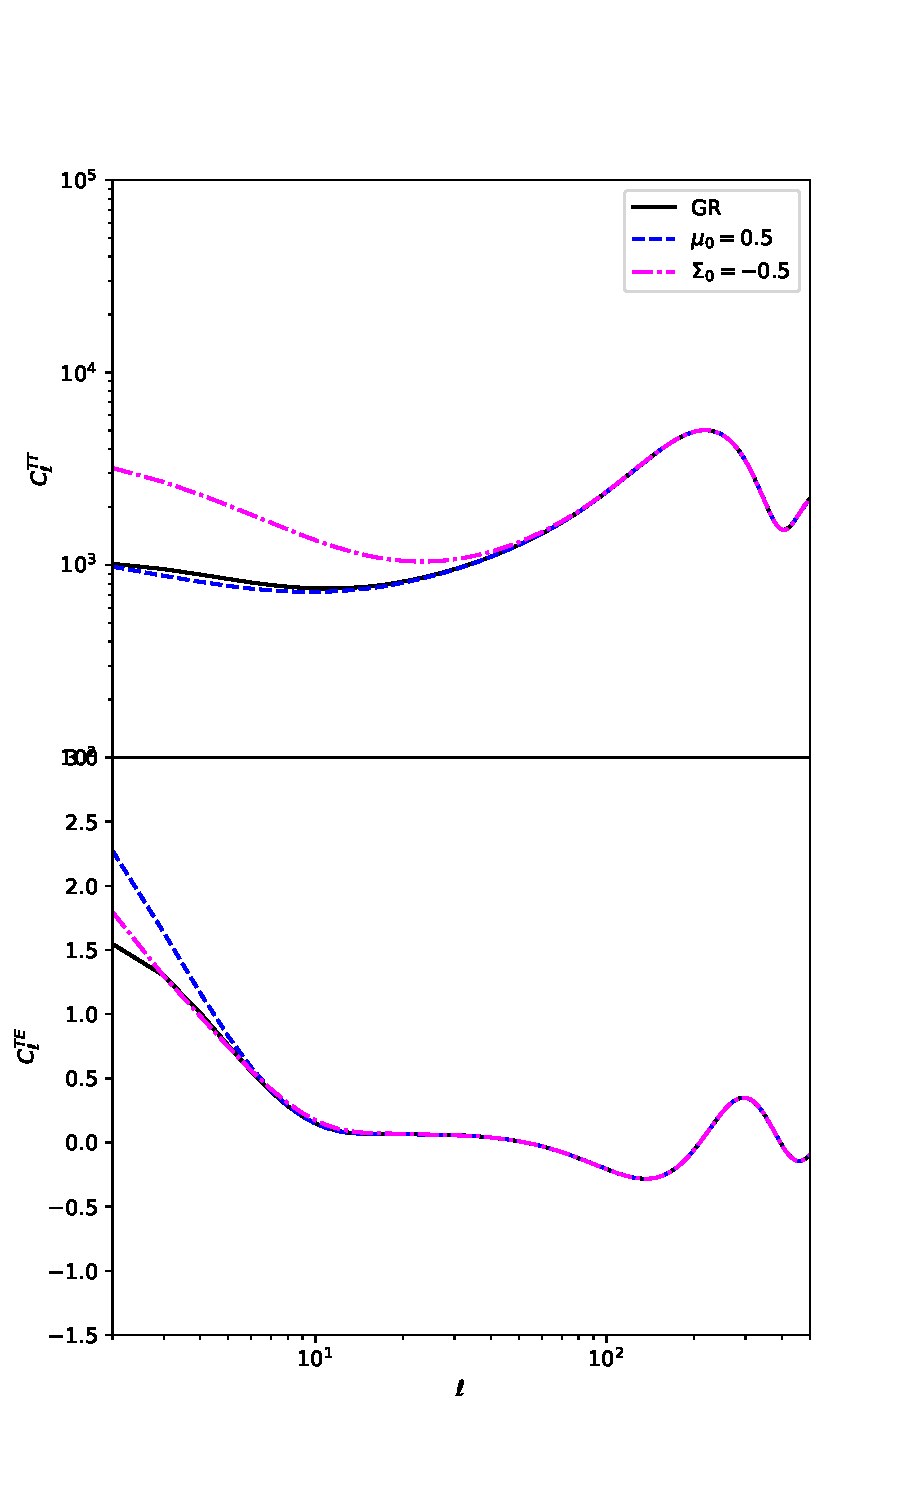
\includegraphics[width=0.5\linewidth]{figures/referee/Fig4_CFHT.pdf}
        \caption{Reproductions of Figures 3 and 4 from CFHTLens, made using CAMB-cs2.}
        \label{fig:reproduction}
    \end{figure}

    \textbf{Comment \#2:} "Since the authors are utilizing the ISW and lensing effects of the CMB, involving scales where QS approximation probably is insufficient, and they already use CAMB, which includes implementation of the full perturbed Einstein equations, I think it may be more appropriate for the authors to use the full equation rather than the QS approximation" \\

    \textbf{Answer \#2:} We thank the referee for this important remark. Indeed, the quasi-static approximation (QSA) is only valid well within the scalar field horizon, that is, $k^2c_s^2 \gg (aH)^2$. Therefore, in our data analysis, we expect this approximation to be insufficient to describe large-scale observables such as the low CMB multipoles, while cosmic shear probes small, subhorizon scales. We have decided to redo our analysis without the QSA, and making a section where we compare the new results with what we had obtained previously. \\

    The main difference is that now, without the QSA, $\mu(k, a)$ can have a pole whenever the denominator of equation (17) is zero. This effectively sets an additional prior that cuts off a big part of the "phantom-crossing" region of the (w0, wa) space.

    \textbf{Comment \#3:} "Fig. 3, I am confused about that lowering $c_s^2$ increases matter power on large scales as in Fig. 2, but decreases lensing power in Fig. 3. It is better to provide more explanation in relevant text." \\

    \textbf{Answer \#3:} Indeed, the referee's intuition is correct. However, the visualization in Figure 2 does not clearly show the effect of $c_s^2$ on small scales: on the right column, all shades of red seem to be equal between the three $c_s^2$ values. When plotting the matter power spectrum at a single redshift, shown in Figure~\ref{fig:pk_z0}, the effects of changing the sound speed are more clear: when we lower the value of $c_s^2$, the matter power spectrum at small scales also decreases relative to other $c_s^2$ values. Therefore, the two pictures are consistent. We would like to maintain the current visualization in the paper, as it conveys more information about the matter power spectrum at all relevant redshifts to our analysis.\\

    \begin{figure}
        \centering
        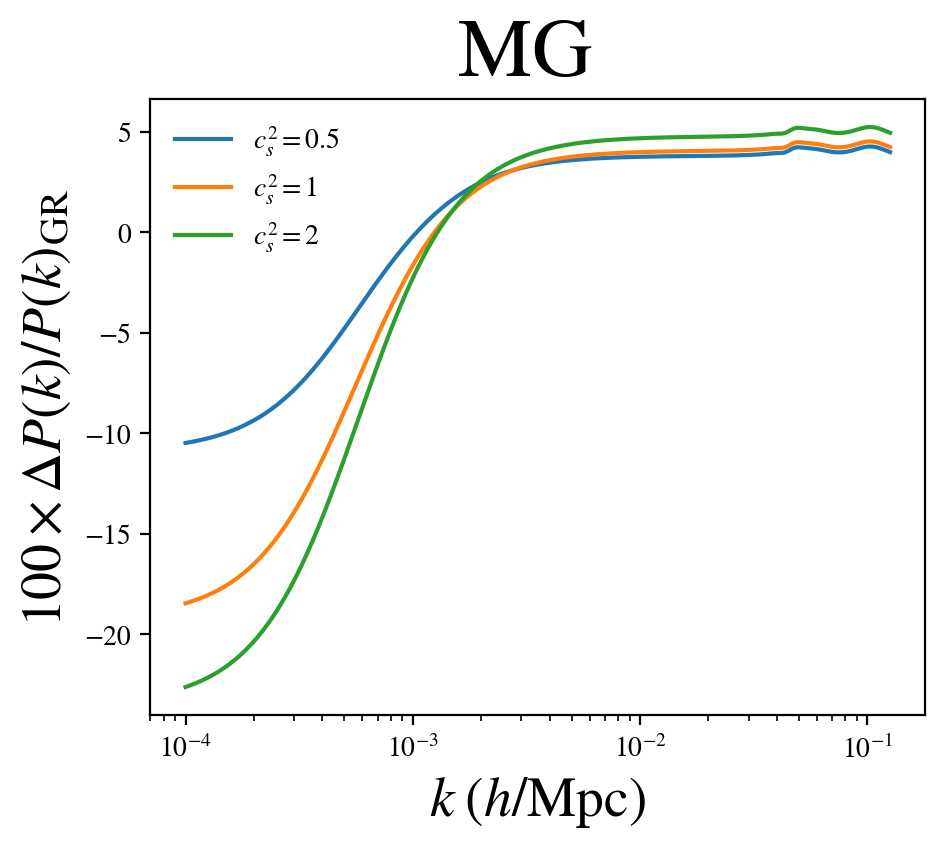
\includegraphics[width=0.5\linewidth]{figures/referee/impact_pk_mg_case1_z0.png}
        \caption{Same as Figure 2 from the paper, but showing a slice at $z = 0$.}
        \label{fig:pk_z0}
    \end{figure}

    \textbf{Comment \#4:} "In the abstract, 'explore correlations between the dark energy sound speed and perturbative behavior', should it be 'correlations between the dark energy sound speed and dynamical behavior'?"\\

    \textbf{Answer \#4:} Indeed, the original phrasing is confusing and the referee's suggestion is in line with the goals of the paper.\\

    \textbf{Comment \#5:} "Eq(3), should explain what prime here stands for."\\

    \textbf{Answer \#5:} Indeed, there had been no mentions to the notation of primes as derivatives with respect to conformal time; we added this explanation in the new version. \\
    
    \textbf{Comment \#6:} "There are several evident mistakes/typoes existing in the manuscript. e.g. 1). In the abstract, the SN data is Pantheon+, while in the main text, it is DES-Dovekie; 2). Caption of Fig. 1, 'in the case of $\alpha_K$', expression incomplete here, so the case is not specified actually. 3). Unit of neff should be $\mathrm{arcmin}^{-2}$. 4). Caption of Fig. 7 mentions blue and orange histograms, but the actual colors are grey and green. Therefore, the authors should carefully check their manuscript." \\

    \textbf{Answer \#6:} We thank the referee for pointing out various mistakes in the draft. We have fixed all of the mistakes mentioned, and proof-read the main text as well as Figure/Table captions to ensure consistency. \\

    We hope the clarifications above address all concerns raised by the referee. \\

    Best, \\
    
    The Authors
    
\end{document}